\section{BLE library on the device}
\subsection{Environment setup}
We program the nRF52840 board using VS Code (Microsoft Visual Studio Code) with PlatformIO IDE extension.
First, we configured the PlatformIO configuration file (platformio.ini) for our project:
\begin{itemize}
    \item \textbf{platform}: the system on chip (SoC) used our board is \textit{nordicnrf52}.
    \item \textbf{board} : the development board we use is \textit{nrf52840\_dk}.
    \item \textbf{framework} : the software environment that runs our project code is \textit{arduino}.
\end{itemize}
Then, since we want to establish a data transmission between the device and the android app via a BLE connection, we add in this configuration file the two necessary parameters : 
\begin{itemize}
    \item \textbf{build\_flags} : the compiler must generate the code with the flag \textit{-DNRF52\_S132}.
    \item \textbf{lib\_deps} : \textit{sandeepmistry/BLEPeripheral@0.4.0} is an arduino library for creating custom BLE peripherals with this board.
\end{itemize}
\subsection{Use of the BLEPeripheral library}
We first import the Arduino library to create custom BLE peripherals (BLEPeripheral) which depends on SPI (Serial Peripheral Interface) library allowing the communication.
Then we define 
\begin{itemize}
    \item pin 14 for the sensor pin (details in section \ref{GPIO14})
    \item a timer variable
    \item an interval at which we send data (in milliseconds)
\end{itemize}
We then proceed to create the misc structured model according to ArduinoBLE \cite{b3}.
\begin{figure}[!ht]%
    \centering
    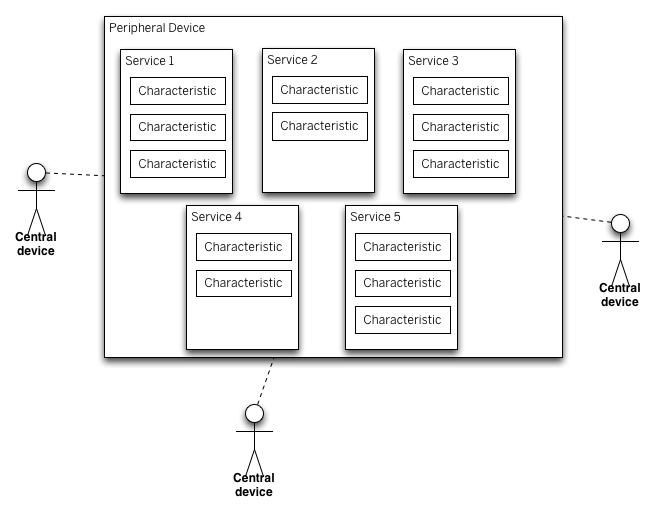
\includegraphics[scale=0.2]{images/ble-bulletin-board-model.png}%
    \caption{ArduinoBLE model}%
    \label{fig:ArduinoBLE}%
\end{figure}
Considering this scheme [Fig. \ref{fig:ArduinoBLE}], we initialize a BLEPeripheral object acting as the peripheral device, a BLEService and a BLECharCharacteristic objects acting as the DHT11 sensor service for temperature characteristic which we specify with a UUID generating from the Internet.
We enable the NOTIFY property of the characteristic: when the sender writes to it, the new value is automatically sent to the receiver (the android app), without the receiver having to issue an explicit read command.

We create callback functions for central connect and disconnect event, for characteristic subscribe and unsubscribed event.

The setup() function initializes and defines the initial values: set sensor pin, assigns the service and characteritic to the device, assign event handlers ...
Finally, the loop() function starts the peripheral, handles the callbacks, read the analog input and save it in the characteristic (in hexacimal format) according to a timer function.